\chapter{}
We left the hotel and headed to the park. Despite the limp caused by her cast, Monique's
pace was very quick. We made our way to park operations, where we rented a wheelchair, and
received our paperwork for special access. Her pass allowed us to bypass the lines completely
for most rides. For the most popular rides, we were given a time to come back, and when we
returned, we were able to get right on.

She got a lot of looks from people in the park. I noticed several of the guys doing double
takes at her, and found myself wondering if they were looking at her because of her cast, of
simply because she was so beautiful.

Riding the roller coasters was great. The coasters there are among the very best in the
world. Her cast presented a few minor problems for us getting into and out of the cars. On a few
of the coasters, the foot space was so limited that she had problems getting the cast into a
comfortable position. The most interesting event on a ride was on the Raptor, a coaster where
the track is above the car and your feet dangle below. On that ride, the attendants asked that
she sit in the seat on the far left. I assume that was so that her cast wouldn't swing around
and hit someone.

\begin{thought}
Monique was having the time of her life. Being pushed around in the wheelchair was great.
She felt very pampered by Quinn, who seemed to be having a lot of fun, too. The wheelchair also
drew a lot of attention, and she had to admit to herself that she enjoyed the attention. She
found herself wondering if any of the men she noticed looking at her two, three, or more times
was in fact, a closet caster. The coasters were awesome, the park was beautiful, and the smell
of the lake was scintillating. As the night wore on, and the park neared closing for the day,
she knew there was one thing left that they had to do.
\end{thought}

``Quinn, let's go turn the wheelchair in, and go for a walk on the beach.''

The idea seemed great to me. It wasn't the ocean, but Lake Erie is big enough to feel like
it. The evening was beautiful, Monique was beautiful, and the beach was the perfect place to
wind up our evening out.

``That's a great idea, let's do it.''

I wheeled her back to guest relations, we turned in the wheelchair, and we headed for the
beach. It was a fair distance, and though she kept up a quick pace as she limped along, I found
myself concerned for Monique's casted foot. I didn't want her to end up with a blister.

``How's the foot doing?'' I asked. ``It isn't hurting, is it?''

``No, it's fine,'' she said. ``The cast shoe is pretty soft- it feels as soft as wearing a
sneaker.''

``Okay- just checking.''

\begin{thought}
``He thinks of everything,'' she thought to herself. The level of thoughtfulness that Quinn
showed to her was one of the things she found herself coming to love about him. She was also
discovering that his unselfish concern for her was making her open herself more to him. She
thought back to only a couple of months ago, when she was very emotionally withdrawn. She hadn't
been a cold, unfeeling person then, she just kept a very solid wall between her heart and the
world. That was then. She had first noticed that she was unable to stop Quinn from reaching her,
and then she noticed that she didn't want to keep him from it. As they reached the beach, and
walked out onto the sand, the moment became one she didn't want to end.
\end{thought}

Walking along the beach with Monique was great. We walked half the length of the beach
without even speaking. That was something about Monique that I had never experienced with anyone
before- long silences were not uncomfortable. Neither of us felt the need to entertain or be
entertained, just being together was enough. We walked past the beach chairs, most of them
empty, a few occupied by sunburned parents as their children ran along and stomped the remains
of the days sand castles. It was Monique who finally broke the silence:

``Oooh, I wasn't expecting THAT.''

``What?''

``Sand in the cast.''

``Ouch,'' I replied. ``We should have thought of that. Is it really uncomfortable?''

``No,'' she answered. ``It's not too bad. I don't want to walk forever like this, but I
wouldn't trade this walk for anything.''

``We'll get you out of that cast as soon as we get back to the room,'' I said, then added ``I
wouldn't trade it, either.''

She smiled, and gave me a quick kiss. We continued walking along the beach until we got
close to the lighthouse. We stopped and watched the light blinking out over the lake for a
while. As we stood there with arms around each other, I was lost in the sensations. The rhythmic
blinking of the light, reflected on the calm surface of the lake; the smell of the water, mostly
pleasant; the sound of the waves licking at the sand; the coolness of the night air, offset by
Monique's warmth pressed hard against my left side.

I honestly could not tell you how long we stood there. It may have been a few minutes, or it
may have been a half hour. Time wasn't too important at that point, and I didn't bother to
check.

It was again Monique who turned to me and broke the silence.

``Quinn, let's head back to the hotel,'' she said.

``Okay, let's get you out of that cast.''

``And into another one?'' she asked with a smile.

``If you like, absolutely,'' I answered.

``Or two, or three?'' she added with an impish smile.

I laughed at her. ``You're incorrigible,'' I told her.

``Count on it!''

After we'd made our way back to the hotel, we went into the bathroom, and cut the cast from
her leg. We did it over the bathtub, so a quick splash of water from the faucet took care of the
cleanup. We decided to leave her uncasted until after we'd eaten dinner, which we ordered from
room service.

Over dinner we recalled the day, and the fun we'd had. We talked of the coasters we'd
ridden, and what we wanted to ride tomorrow. We were truly having a great time together. As the
conversation unfolded, I began to realize that this was a fantastic trip in every regard. I also
realized that the fact that she'd spent most of the time in a cast was not the high point of the
trip. It was wonderful, without a doubt; but the trip and the company would have been wonderful
without any ``hardware.''

As we finished dinner, we stayed seated at the table, talking. Monique brought up the
subject. ``So, when do I get my new cast?''

``Anytime you'd like. If you want it tonight, we can do it whenever. If you'd like a free
evening, we can wait until tomorrow morning. Or skip it entirely.''

``Skip it entirely? Perish the thought!'' she answered playfully. ``What kind of cast model
would I be if I wimped out on you, now?''

I shook my head. ``Monique, I think you're slightly more than a model, now.'' I looked her in
the eye. ``At least I'm hoping you are. I'm having a great time with you. We can pack up the
supplies and just hang out together. I would have the time of my life with you whether or not we
cast you.''

I wish I could have described the warmth in the smile that she broke into at my comment.
She didn't answer my statement immediately. She got up, and walked around the table to my side.
She turned me to face her. She then climbed onto my lap, facing me, with her legs wrapped around
me.

``I'm very glad to hear that, I really am. I'm having the time of my life with you, too, and
I enjoy wearing the casts, for several reasons. I'd hate it if the only reason you wanted to be
with me was for the way I fill up a cast.''

``Monique,'' I replied, ``it isn't.''

She smiled again. ``And I know that.'' We melted into a long, passionate kiss that lasted…
well; I really couldn't tell you for sure how long it lasted. It might have been a minute, it
might have been ten minutes. Hell, it might have been more- time wasn't the issue at that
moment.

After the kiss, we just sat there, gazing at each other for a few moments. Monique spoke
first. ``But, any woman who doesn't like to dress to please her man doesn't deserve him, now
does
she?'' She asked with the familiar, playful smile.

I couldn't help but smile back. ``Well, it's nice, but I hardly think it's the key element in
a good relationship.''

She rolled her eyes and shook her head in mock disgust.'' So, am I going to have to cast
myself, now that you're all serious?''

``No, ma'am, I'll be happy to oblige your needy leg. Is your ankle hurting much?''

``It hurts quite a bit, but it's not near as bad as my arms.'' She said, dangling both arms
like dead weight.

``Arms?'' I asked with eyebrow lifted.

``Yes, they're in agony. It's like they are on fire- my shoulders, too. ''

I was stunned, and it must have showed on my face.

``What's the matter?'' she asked. ``I know from firsthand experience that you can make a nice
shoulder spica. What's so hard about adding in the other arm?''

``Nothing, really. I'm up for it if you're sure you are.''

``Eh, I've worn bigger,'' she retorted nonchalantly.

I smiled at her. ``Anything the lady wishes will be my happiest duty.'' And started opening
up the supplies. Fortunately, I really HAD packed us heavy on goodies. While a double shoulder
spica would seriously dent the mini-stash we had, it wouldn't exsanguinate the supply.

She brought her chair over to where I was, and sat in front of me, holding her left leg out
toward me. ``The leg first doctor, if you please.''

``Let's head to the bathroom,'' I said, pulling on a pair of gloves.

\begin{thought}
Monique watched as Quinn smiled, and began to cast her leg. Though having him wrap padding
and fiberglass on her was nothing new, she still enjoyed it more each time he did it. The leg
cast was nothing major, just a well padded short leg cast for tomorrow's venture into the park.
He worked quickly, but skillfully. After a few minutes, he was pulling off his gloves and they
both admired his work. It felt good, it looked good, and she was seriously anticipating what
came next. They shared a smoke, and as soon as they were finished, he gloved back up, and
slipped her tank top off. She found herself secretly hoping he would take off her bra as well,
but he did not, and she knew why- the bra would help keep her breasts from flattening under the
cast as it was applied. He cut a section of the large stockinette and slid it over her down to
her hips. He then pulled it up to her armpits, and then slit it on each side so he could pull it
up in the front and back, securing it to itself over each shoulder. He then cut two long
sections of the smaller stockinette and pulled them up first the left arm, then the right.

He started wrapping padding on the left arm, and wrapped it from her hand to her upper arm.
He then repeated the process on the right. He got some wider padding, and wrapped from just
below her waist upward, covering her to her armpits. Then, back to her arms, wrapping the top of
each arm, and shoulder. Monique looked away from Quinn's working on her. There was a full length
mirror on the bathroom door, and she watched him work through the reflection as her upper body
became soft-looking and snowy white.

After the padding was done, Quinn put on his gloves and ripped open a roll of pink
fiberglass. He began wrapping her left hand, and worked his way up her arm. After the first roll
was finished, he went back and anchored the padding and stockinette at the hand, and then
proceeded up the arm. A few rolls later, he was wrapping the shoulder and around her chest. With
the left arm finished, he repeated the process on the right arm. It was a bit tiring, holding
her arms out at her sides, but it did not detract from the exhilaration that she felt at the
cast application. As always, getting the cast applied was a sensory treat: the smell of the
fiberglass; the gentle sound of the wet fiberglass as he pulled it from the roll as he wrapped;
the vision in the mirror of him working as her body became more and more encased in the setting
pink shell. Most of all, she enjoyed the sensation of gentle and slight pressure as he wrapped
and molded the material on her body.

When he had finished the cast by anchoring it at her waist, he pulled off the gloves and
stepped back to admire his work. The satisfied smile on his face told Monique that Quinn liked
what he saw.
\end{thought}

Monique looked unbelievable in her casts. The short leg cast was molded very well. It did
not hide the beautiful shape of her leg, but merely accentuated it. The double shoulder spica
was fantastic, if I did say so myself.

We waited a few minutes while the cast dried. I went and retrieved the cast shoe, and put
it on her casted left foot. I helped her to stand, and then steadied her as she walked into the
bedroom. I helped her into bed, and went to get my sketchpad. I was starting to feel a bit
tired, but I couldn't wait to draw her like this.

\begin{thought}
As she sat on the bed, watching Quinn work over his paper, Monique was enjoying the feel of
the huge cast. She found she could twist a slight bit inside the cast, but not much. She was
truly held fast from her waist to her neck, and it was wonderful. She was totally helpless and
dependent on this man she was falling in love with, and it was a wonderful feeling. She was
surprised to be able to admit to herself that she was falling in love, but the self-realization
felt good. The fact that she found herself able to trust him when she was so unable to help
herself warmed her from the inside. Although they couldn't do it now, she wondered what it would
be like to be out in public in a cast this massive. It seemed that everyone noticed her when she
was wearing just the short leg cast. What would it be like if she was out like this? She just
might have to bring it up to Quinn sometime. It was one of the things that they could do down
the road. She hoped that road was a long one.
\end{thought}

When I was done with the sketch, I glanced at my watch and couldn't believe how late it had
gotten. No wonder I felt tired. I noticed Monique had a sleepy look in her eyes as well, so I
helped her into bed, and then got in myself. I kissed her goodnight, and cuddled into embrace
her as best I could. I found that if I lay a pillow on her upper arm, I could rest my head on
that. I slipped one arm underneath the pillow she had her head on, and laid the other arm across
her casted midsection. It wasn't long before I was asleep.

\begin{center}
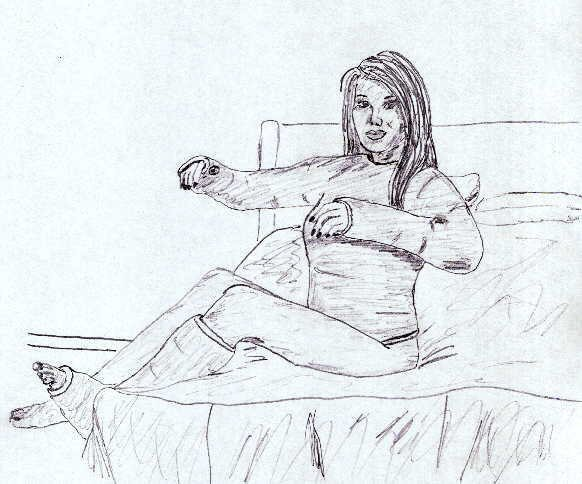
\includegraphics{images/kicks30.jpg}
\end{center}
